\section{Umsetzung virtueller Spiele in der physischen Welt}

Unter einem virtuellen Spiel verstehen wir jene, die sich ausschließlich mit bzw. auf einem Computers spielen lassen. \newline
Es folgen eine Reihe von Spielideen, die in der virtuellen Welt sehr populär sind und sich für die Integration in die physische Welt eignen.
\subsection*{Snake}
Ein absoluter Klassiker, der früher auf keinem Handy fehlen durfte. Gerade wegen der
Popularität und Einfachheit recht interessant es in die physische Welt zu integrieren.
In einem begrenzten Areal gilt es eine Schlange geschickt zu steuern. Es müssen kleine
Items eingesammelt werden, wodurch die Schlange wächst. Außerdem muss darauf
geachtet werden, dass weder der Rand des Areals noch die eigene Schlange berührt wird.
\newline
Snake ist ursprünglich ein Einzelspieler-Spiel, da es unüblich ist, Outdoor-Bewegungsspiele allein zu spielen, haben wir entschieden Snake in der physischen Welt als Mehrspieler-Spiel umzusetzen.

\begin{figure}[htbp]
  \centering
    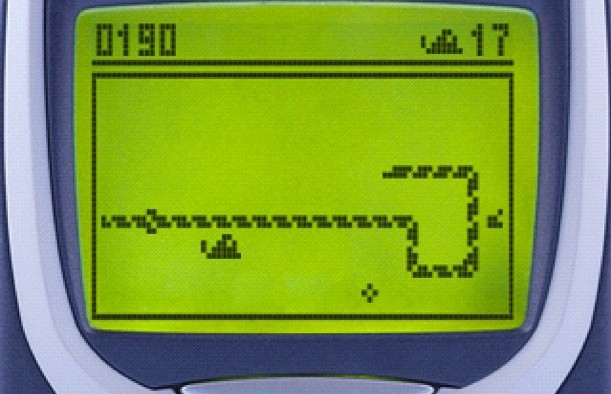
\includegraphics[width=0.5\textwidth]{2-Spielideen/2-1-Umsetzung_virtueller_Spiele_in_der_physischen_Welt/snake.png}
     \caption{Snake auf dem Nokia 3310 
		(Quelle: \url{http://nixtv.de/wp-content/uploads/2014/09/snake.jpg}) }
\end{figure}

\subsection*{Capture the Flag}
Das Spiel ist nicht nur in der virtuellen Welt spielbar, wurde dort aber erst richtig bekannt.
Auch hier ist ein recht einfacher Spielmechanismus ausschlaggebend für einen leichten
Einsatz in der physischen Welt.
Zwei Teams treten gegeneinander an. Jedes Team besitzt eine Flagge, dessen Standort für
das gegnerische Team bekannt ist. Es wird versucht die Flagge des jeweils anderen Teams
zum Standort der eigenen Flagge zu bringen.
\subsection*{Domination}
Meist in Kriegsszenarien integrierter virtueller Spielmodi, der sich mit wenig Aufwand in die
physische Welt übertragen lässt.
Zwei Teams treten gegeneinander an. Jedes Team hat einen Punktestand, der zu Anfang
gleich ist. Sinkt der Punktestand auf Null, so ist das Spiel für dieses Team verloren. Es gibt
verschiedene Areale, die eingenommen werden können. Hat ein Team mehr Areale
eingenommen als das andere, läuft der Punktestand des Teams, das weniger Areale in
besitzt hat schneller gegen Null.
